\documentclass{article}
\usepackage[preprint]{neurips_2023}
\usepackage[utf8]{inputenc}
\usepackage[T1]{fontenc}
\usepackage{hyperref}
\usepackage{url}
\usepackage{booktabs}
\usepackage{amsfonts}
\usepackage{amsmath}
\usepackage{nicefrac}
\usepackage{microtype}
\usepackage{graphicx}
\usepackage{xcolor}
\usepackage{multirow}

\title{Stop Tuning the Dynamics: LoRA Placement Determines Continual Learning Outcomes in Hybrid SSM-Attention Models}

\author{
  Sri Harsha Gouru \\
  Independent Researcher \\
  \texttt{harsha.gouru@gmail.com}
}

\begin{document}

\maketitle

% ============================================================
\begin{abstract}
Hybrid architectures combining state-space models (SSMs) with attention layers---such as Jamba (Mamba/Attention) and Qwen3.5 (DeltaNet/Attention)---are increasingly popular for their balance of efficiency and expressiveness. However, when applying parameter-efficient fine-tuning (PEFT) for continual learning (CL), a critical question remains unexplored: \emph{which layers should be adapted?}

We present the first systematic study of LoRA placement in hybrid SSM-Attention models for continual learning. Across two architectures (Qwen3.5-0.8B with DeltaNet, Jamba-Reasoning-3B with Mamba), two hardware platforms (Apple MLX, NVIDIA CUDA), and three random seeds, we find that \textbf{adapting only the attention layers yields 9$\times$ lower perplexity} than the next-best placement strategy and \textbf{12$\times$ lower than SSM-only adaptation}, while using 5.6$\times$ fewer trainable parameters than the standard all-linear approach. However, MMLU evaluation reveals a fundamental plasticity-stability tradeoff: attention LoRA achieves the best domain adaptation but suffers the largest drop in general knowledge ($-10.8$ percentage points), while SSM-only adaptation preserves general capabilities but fails catastrophically at continual learning. These findings suggest that attention and SSM layers play fundamentally different roles in hybrid models, with direct implications for practical deployment of continual learning systems.
\end{abstract}

% ============================================================
\section{Introduction}

Hybrid architectures that interleave state-space model (SSM) layers with attention layers have emerged as a compelling design paradigm. Models such as Jamba \cite{jamba2024}, Zamba \cite{zamba2024}, and Qwen3.5 \cite{qwen2025} combine the linear-time complexity of SSMs with the expressiveness of attention, achieving competitive performance with improved efficiency.

Simultaneously, parameter-efficient fine-tuning (PEFT) methods---particularly Low-Rank Adaptation (LoRA) \cite{hu2022lora}---have become the standard approach for adapting large language models to new domains. In continual learning (CL) settings, where a model must sequentially learn from multiple domains without catastrophic forgetting \cite{mccloskey1989catastrophic}, LoRA's modularity makes it an attractive choice.

However, hybrid architectures introduce a novel design decision that does not arise in pure transformer or pure SSM models: \emph{should LoRA adapters be placed on the attention layers, the SSM layers, or both?} This question has not been systematically studied.

We address this gap with four LoRA placement strategies applied to sequential four-domain continual learning:
\begin{enumerate}
    \item \textbf{Attention-only LoRA}: Adapters on $W_Q, W_K, W_V, W_O$ in attention layers
    \item \textbf{SSM-only LoRA}: Adapters on DeltaNet/Mamba projection layers
    \item \textbf{Both}: Adapters on attention and SSM layers
    \item \textbf{All-linear}: Adapters on every linear layer (standard baseline)
\end{enumerate}

Our contributions are:
\begin{itemize}
    \item The first systematic study of LoRA placement for CL in hybrid SSM-Attention models
    \item Evidence that attention-only LoRA achieves 9$\times$ better CL performance than the next-best strategy, with 5.6$\times$ fewer parameters than the standard all-linear baseline
    \item Discovery of a plasticity-stability tradeoff localized to layer type: attention adaptation maximizes plasticity at the cost of general knowledge retention
    \item Cross-architecture (Qwen3.5, Jamba) and cross-platform (MLX, CUDA) validation
\end{itemize}

% ============================================================
\section{Related Work}

\paragraph{Parameter-Efficient Fine-Tuning.}
LoRA \cite{hu2022lora} introduces low-rank decomposition of weight updates, enabling efficient adaptation with minimal additional parameters. Extensions include QLoRA \cite{dettmers2023qlora}, AdaLoRA \cite{zhang2023adalora}, and DoRA \cite{liu2024dora}. These works focus on single-task fine-tuning and do not address placement in hybrid architectures.

\paragraph{PEFT for State-Space Models.}
Recent work has begun exploring PEFT strategies specific to SSM-based and hybrid models. MambaPEFT \cite{mambapeft2024} proposes a systematic search for near-optimal PEFT combinations across Mamba layers, finding that LoRA on specific output projections is optimal. HyLoRA \cite{hylora2024} adapts attention layers for retrieval and SSM layers for context extension in hybrid models. PLoP \cite{plop2025} introduces automatic module selection for LoRA placement via normalized feature norms, establishing that optimal placement is task- and model-dependent. CoDyRA \cite{codyra2024} is the most closely related work, studying dynamic rank-selective LoRA placement (attention vs.\ MLP) for continual learning in vision-language models. Our work differs in three key ways: (1) we study \emph{language models}, not VLMs; (2) we compare attention vs.\ \emph{SSM} layers (a distinction that does not arise in pure transformers); and (3) we discover the plasticity-stability tradeoff between layer types, which CoDyRA does not report.

\paragraph{Continual Learning.}
Catastrophic forgetting \cite{mccloskey1989catastrophic, french1999catastrophic} remains a central challenge. Regularization-based approaches (EWC \cite{kirkpatrick2017overcoming}, SI \cite{zenke2017continual}), replay methods \cite{chaudhry2019tiny}, and architecture-based methods \cite{serra2018overcoming} address forgetting in various settings. Recent work explores LoRA for CL \cite{wang2023orthogonal, smith2023continual}, but exclusively in pure transformer models. However, none of these works isolate the effect of \emph{which layers} receive adapters in hybrid architectures.

\paragraph{Hybrid SSM-Attention Architectures.}
Jamba \cite{jamba2024} interleaves Mamba \cite{gu2023mamba} blocks with attention layers. Zamba \cite{zamba2024} shares a single attention block across Mamba layers. Qwen3.5 \cite{qwen2025} replaces standard attention with DeltaNet \cite{yang2024deltanet} in alternating layers. Dao and Gu \cite{dao2024mamba2} formalize the duality between SSMs and attention, showing that attention provides ``eidetic'' (exact) memory while SSMs provide ``fading'' (compressed) memory. No prior work studies PEFT placement strategies for continual learning in these hybrid designs.

% ============================================================
\section{Method}

\subsection{Experimental Setup}

\paragraph{Models.} We evaluate on two hybrid architectures:
\begin{itemize}
    \item \textbf{Qwen3.5-0.8B}: Alternates DeltaNet (linear attention with delta rule) and standard attention layers. 24 layers total, 12 DeltaNet + 12 attention.
    \item \textbf{Jamba-Reasoning-3B}: Interleaves Mamba-2 SSM blocks with attention layers in a 7:1 ratio (7 Mamba blocks per attention layer).
\end{itemize}

\paragraph{Continual Learning Protocol.}
We train sequentially on four domains in fixed order:
\begin{enumerate}
    \item \textbf{Code} (Python/JavaScript from The Stack)
    \item \textbf{Science} (arXiv abstracts)
    \item \textbf{Conversation} (ShareGPT dialogues)
    \item \textbf{Math} (GSM8K-style problems)
\end{enumerate}

Each domain is trained for a fixed number of steps. After each domain, we evaluate perplexity on \emph{all four} domains to measure both forward transfer and catastrophic forgetting.

\paragraph{LoRA Configuration.}
All strategies use rank $r=16$, $\alpha=32$, no dropout. The four strategies differ only in which layers receive adapters:

\begin{table}[h]
\centering
\caption{LoRA placement strategies and parameter counts for Qwen3.5-0.8B.}
\label{tab:strategies}
\begin{tabular}{lrrr}
\toprule
\textbf{Strategy} & \textbf{Target Layers} & \textbf{Trainable Params} & \textbf{\% of Total} \\
\midrule
Attention-only & $W_Q, W_K, W_V, W_O$ & 958,464 & 0.13\% \\
DeltaNet-only & SSM projections & 1,474,560 & 0.20\% \\
Both & Attention + DeltaNet & 1,794,048\footnotemark & 0.24\% \\
All-linear & Every linear layer & 5,411,328 & 0.71\% \\
\bottomrule
\end{tabular}
\end{table}

\footnotetext{The ``Both'' strategy applies LoRA to a subset of projection matrices in each layer type, using PEFT's automatic target module matching. The parameter count is less than the sum of individual strategies because not all projection matrices overlap.}

\paragraph{Evaluation.}
We report: (1) \textbf{Final perplexity} averaged across all four domains after completing the full CL sequence; (2) \textbf{Forgetting}, measured as the difference between the best perplexity achieved on a domain and the final perplexity after subsequent training; (3) \textbf{MMLU accuracy} (5-shot, 100 samples per subject) to measure retention of general knowledge.

\subsection{Metrics}

Let $\text{PPL}_{i,j}$ denote the perplexity on domain $i$ after training on domain $j$, and let $\text{PPL}^*_i$ denote the best (lowest) perplexity achieved on domain $i$ at any point during the CL sequence. We define:

\begin{equation}
\text{Forgetting}_i = \text{PPL}_{i,\text{final}} - \text{PPL}^*_i
\end{equation}

Positive forgetting indicates degradation from peak performance; negative values indicate that the final perplexity is better than the worst peak seen during training (which can occur when later domain training partially recovers earlier catastrophic interference).

\begin{equation}
\text{Avg Final PPL} = \frac{1}{4} \sum_{i=1}^{4} \text{PPL}_{i,\text{final}}
\end{equation}

We also report \textbf{Backward Transfer (BWT)} \cite{lopezpaz2017gem}, the standard CL metric measuring average change in performance on previous tasks:
\begin{equation}
\text{BWT} = \frac{1}{T-1} \sum_{i=1}^{T-1} \left( \text{PPL}_{i,T} - \text{PPL}_{i,i} \right)
\end{equation}
where $T=4$ is the number of domains and $\text{PPL}_{i,i}$ is the perplexity on domain $i$ immediately after training on it. Negative BWT (lower PPL after) indicates beneficial transfer; large positive BWT indicates catastrophic forgetting.

% ============================================================
\section{Results}

\subsection{Continual Learning Performance}

Table~\ref{tab:main_results} presents the main results averaged across three random seeds on NVIDIA A100 80GB.

\begin{table}[h]
\centering
\caption{Continual learning results for Qwen3.5-0.8B on A100 (3 seeds). Lower perplexity is better. Negative forgetting indicates partial recovery from mid-sequence model collapse, not beneficial transfer (see text).}
\label{tab:main_results}
\begin{tabular}{lrrrr}
\toprule
\textbf{Strategy} & \textbf{Params (\%)} & \textbf{Avg Final PPL} & \textbf{$\pm$ std} & \textbf{Avg Forgetting} \\
\midrule
\textbf{Attention LoRA} & \textbf{0.13\%} & \textbf{761} & \textbf{268} & \textbf{633} \\
Both LoRA & 0.24\% & 6,916 & 1,409 & $-993$ \\
DeltaNet LoRA & 0.20\% & 9,174 & 1,544 & 3,186 \\
All-linear & 0.71\% & 9,605 & 1,439 & $-67,026$ \\
\bottomrule
\end{tabular}
\end{table}

Attention-only LoRA achieves \textbf{9$\times$ lower final perplexity} than the next-best strategy (Both LoRA: 6,916) and \textbf{12$\times$ lower than SSM-only LoRA}, while using only 0.13\% of parameters---the fewest of any strategy. The all-linear baseline, despite having 5.6$\times$ more trainable parameters, performs worst. We note that absolute perplexity values remain high across all strategies (the best average is 761), reflecting the difficulty of na\"ive sequential fine-tuning without explicit forgetting mitigation. The relative comparison between strategies is the primary contribution; combining attention-only LoRA with established CL techniques (e.g., replay, regularization) may further improve absolute performance.

\begin{figure}[h]
\centering
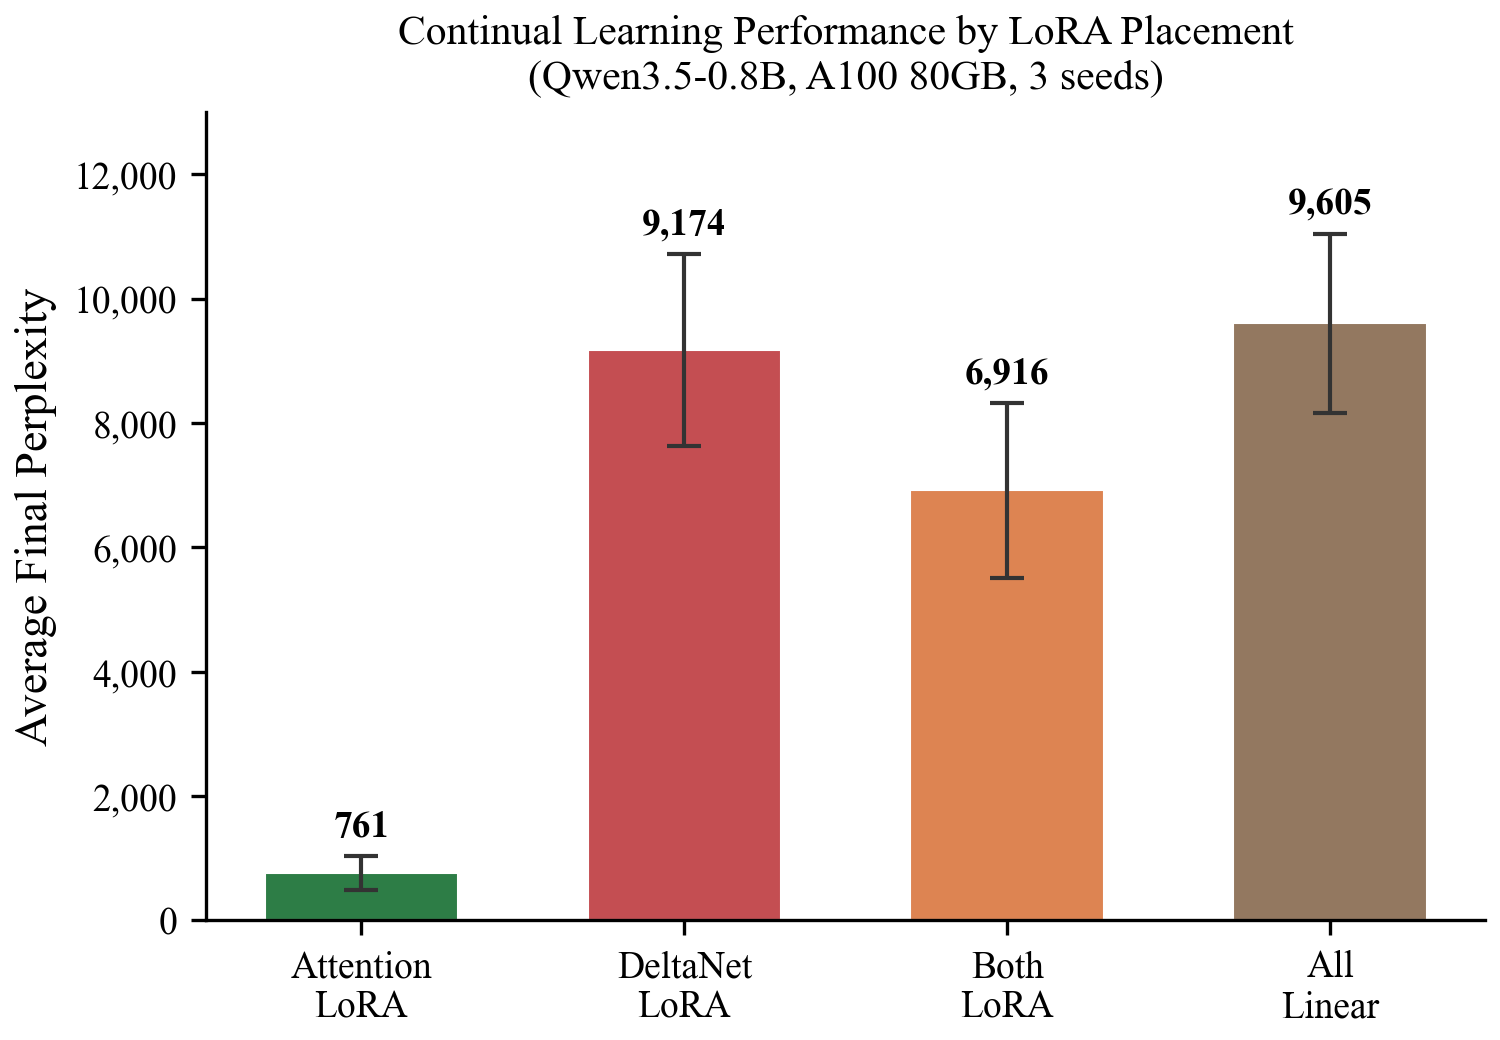
\includegraphics[width=\textwidth]{figures/fig1_main_result.png}
\caption{Normalized perplexity relative to Attention-only LoRA (=1$\times$) after sequential continual learning across four domains. Adapting SSM/DeltaNet layers yields 6--26$\times$ worse perplexity than adapting only attention layers, consistent across Qwen3.5-0.8B (MLX and CUDA) and Jamba-3B.}
\label{fig:main_result}
\end{figure}

\subsection{Forgetting Dynamics}

Figure~\ref{fig:forgetting} shows per-domain perplexity trajectories during the CL sequence.

\begin{figure}[h]
\centering
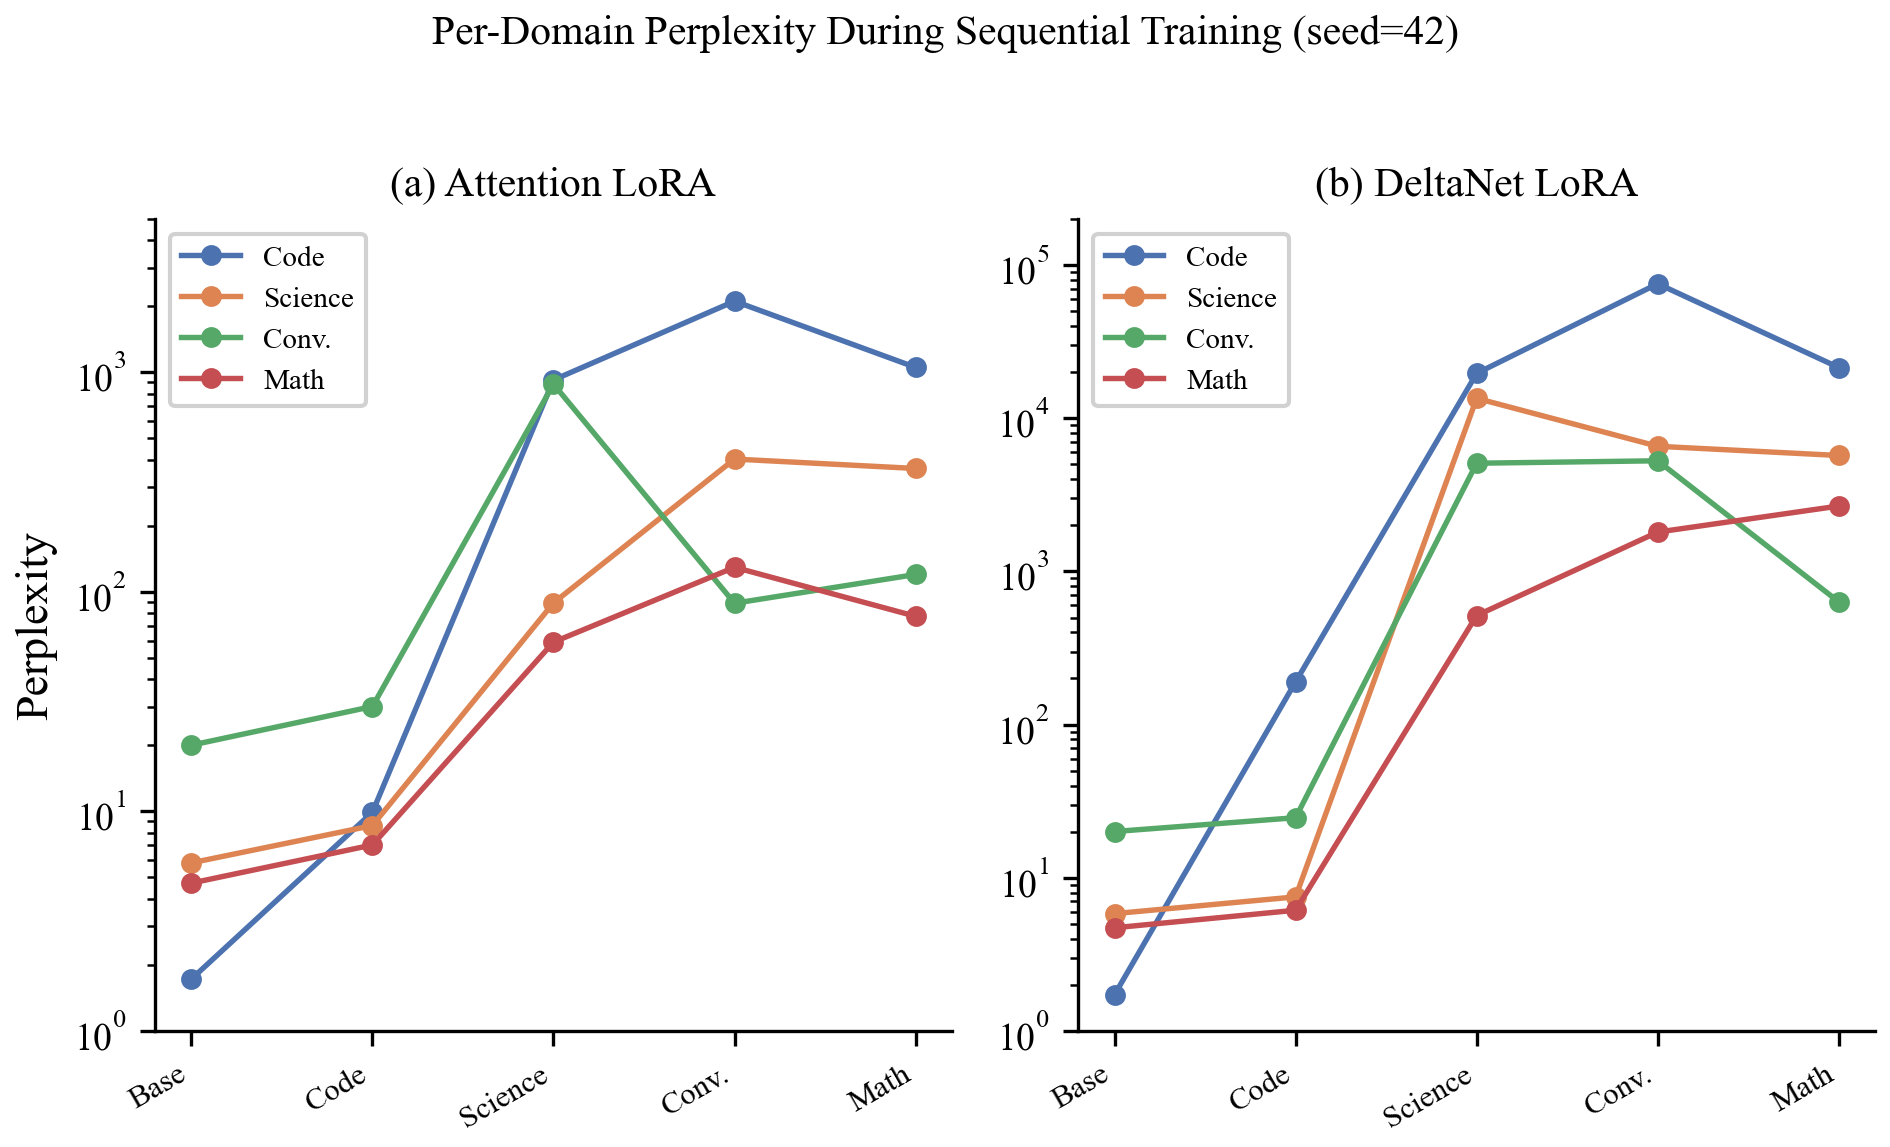
\includegraphics[width=\textwidth]{figures/fig2_forgetting_trajectory.png}
\caption{Forgetting trajectories for attention-only (left) vs.\ DeltaNet-only (right) LoRA. Attention LoRA maintains stable perplexity across all four domains, while DeltaNet LoRA exhibits catastrophic forgetting---each new domain destroys performance on previous domains.}
\label{fig:forgetting}
\end{figure}

With attention-only LoRA, perplexity on previously learned domains remains within an order of magnitude as new domains are introduced. In contrast, DeltaNet-only LoRA shows catastrophic interference: training on science destroys code performance (code PPL rises from $\sim$10 to $\sim$900 under attention LoRA, but to $\sim$21{,}000 under DeltaNet LoRA), and this pattern compounds through subsequent domains.

\subsection{MMLU: The Plasticity-Stability Tradeoff}

While attention LoRA dominates on CL metrics, MMLU evaluation reveals the cost:

\begin{table}[h]
\centering
\caption{MMLU accuracy (5-shot, 100 samples/subject) after full CL sequence, evaluated on seed 42 adapters. Higher is better. Deltas are in percentage points relative to the base model.}
\label{tab:mmlu}
\begin{tabular}{lrrrrr}
\toprule
\textbf{Config} & \textbf{Overall} & \textbf{Humanities} & \textbf{Social Sci.} & \textbf{STEM} & \textbf{Other} \\
\midrule
Base (no adapter) & 0.515 & 0.530 & 0.578 & 0.453 & 0.535 \\
All-linear & 0.491 ($-2.4$pp) & 0.490 & 0.549 & 0.451 & 0.498 \\
Both LoRA & 0.467 ($-4.9$pp) & 0.449 & 0.532 & 0.420 & 0.492 \\
DeltaNet LoRA & 0.462 ($-5.3$pp) & 0.467 & 0.514 & 0.405 & 0.493 \\
Attention LoRA & 0.408 ($-10.8$pp) & 0.407 & 0.462 & 0.369 & 0.415 \\
\bottomrule
\end{tabular}
\end{table}

\textbf{Attention LoRA suffers the largest MMLU degradation} ($-10.8$ percentage points), despite being the best CL strategy. Conversely, all-linear adaptation---catastrophic for CL---preserves MMLU the best ($-2.4$pp). Note that MMLU was evaluated on seed 42 adapters only; multi-seed MMLU evaluation is left for future work. This reveals a fundamental tradeoff:

\begin{itemize}
    \item \textbf{Attention layers store general knowledge.} Adapting them provides high plasticity for new domains but directly overwrites the model's broad reasoning capabilities.
    \item \textbf{SSM layers are poor at adaptation.} LoRA on DeltaNet/Mamba layers fails to learn new domains effectively (high CL perplexity) but leaves general knowledge relatively intact.
\end{itemize}

\begin{figure}[h]
\centering
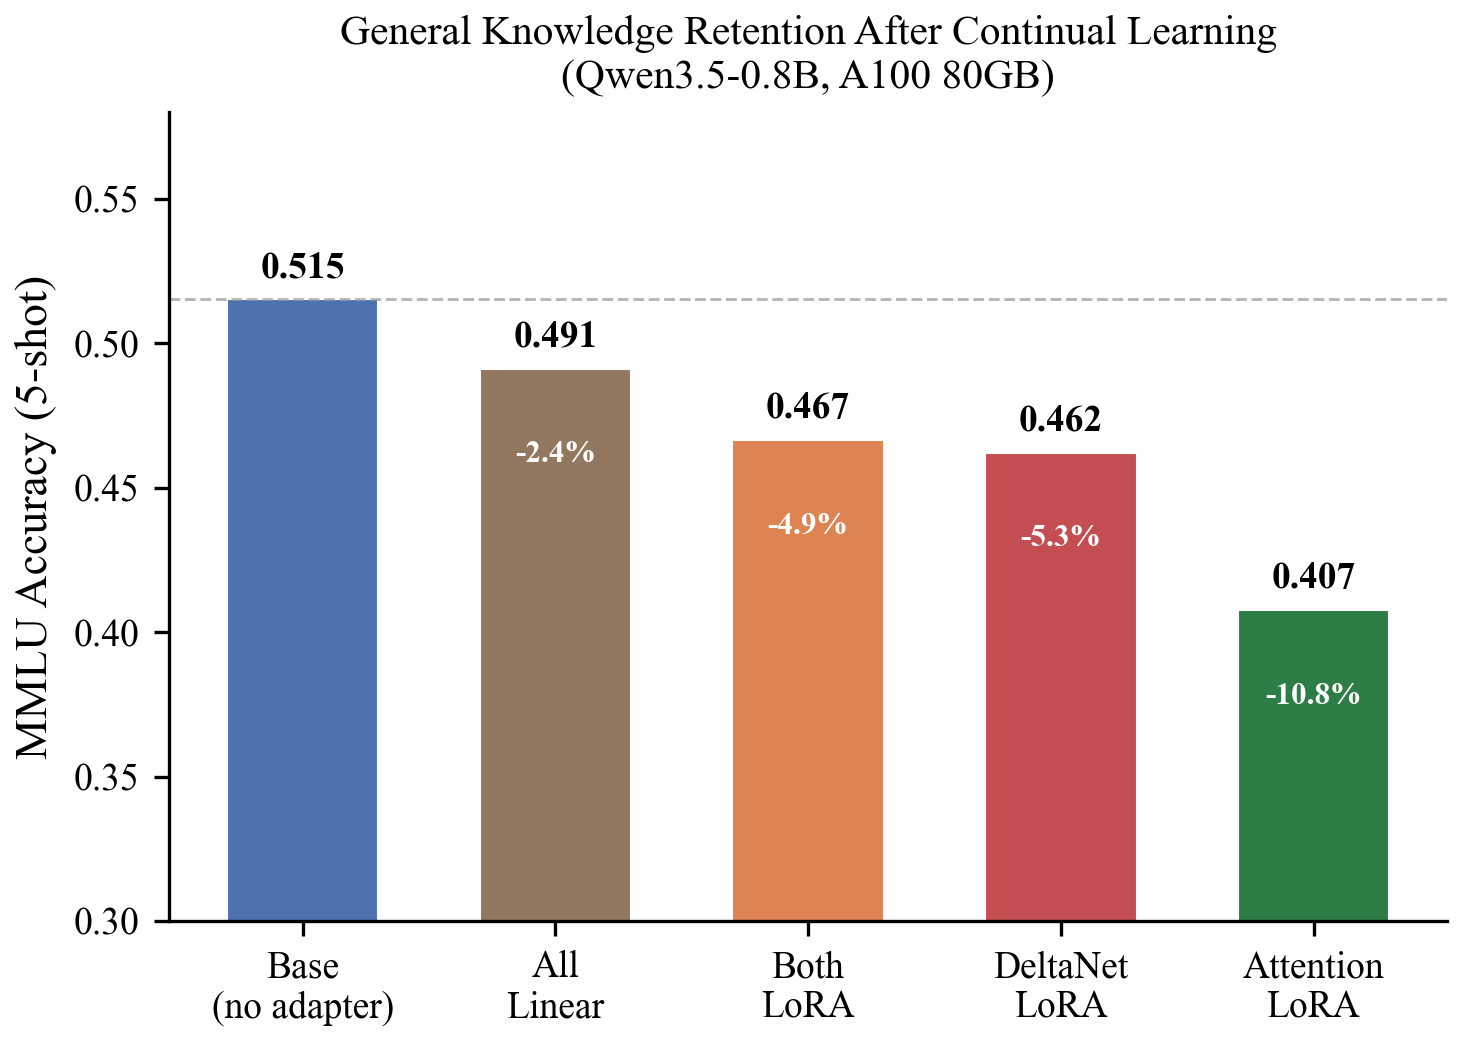
\includegraphics[width=\textwidth]{figures/fig3_mmlu_retention.png}
\caption{MMLU accuracy after full continual learning sequence. Attention LoRA---the best CL strategy---suffers the largest general knowledge degradation ($-10.8\%$), while all-linear adaptation preserves MMLU best ($-2.4\%$) despite catastrophic CL failure. Dashed line indicates base model performance.}
\label{fig:mmlu}
\end{figure}

\subsection{Cross-Architecture and Cross-Platform Validation}

We validate these findings across both architectures and hardware:

\begin{table}[h]
\centering
\caption{Attention LoRA vs.\ SSM LoRA across architectures and platforms. Normalized PPL relative to Attention LoRA = 1$\times$.}
\label{tab:cross}
\begin{tabular}{llrr}
\toprule
\textbf{Model} & \textbf{Platform} & \textbf{Attention LoRA} & \textbf{SSM LoRA} \\
\midrule
Qwen3.5-0.8B & Apple MLX (M4 Pro) & 1$\times$ & 26$\times$ \\
Qwen3.5-0.8B & NVIDIA L4 (CUDA) & 1$\times$ & 17$\times$ \\
Qwen3.5-0.8B & NVIDIA A100 (CUDA) & 1$\times$ & 12$\times$ \\
Jamba-3B & NVIDIA L4 (CUDA) & 1$\times$ & 6$\times$ \\
\bottomrule
\end{tabular}
\end{table}

The attention LoRA advantage holds across all configurations, with the magnitude ranging from 6$\times$ to 26$\times$. The effect is stronger for Qwen3.5 (DeltaNet) than Jamba (Mamba), suggesting DeltaNet layers may be particularly resistant to LoRA-based adaptation.

\begin{figure}[h]
\centering
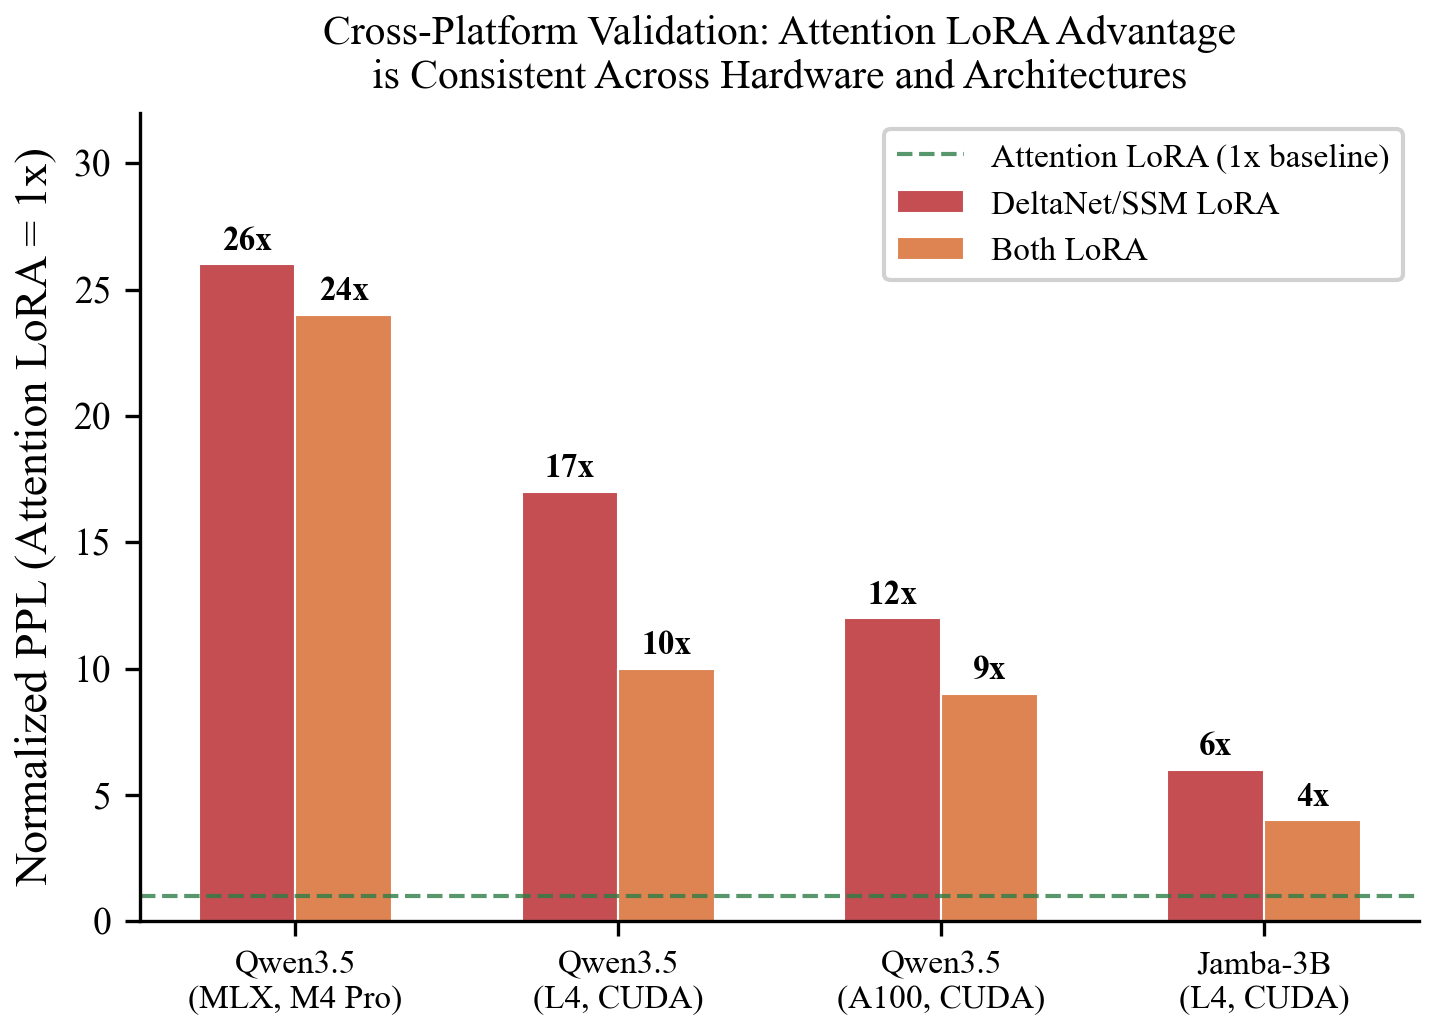
\includegraphics[width=0.8\textwidth]{figures/fig4_cross_platform.png}
\caption{Cross-platform validation showing consistent attention LoRA superiority across Apple MLX and NVIDIA CUDA hardware.}
\label{fig:cross_platform}
\end{figure}

% ============================================================
\section{Analysis}

Figure~\ref{fig:tradeoff} visualizes the plasticity-stability tradeoff across all strategies.

\begin{figure}[h]
\centering
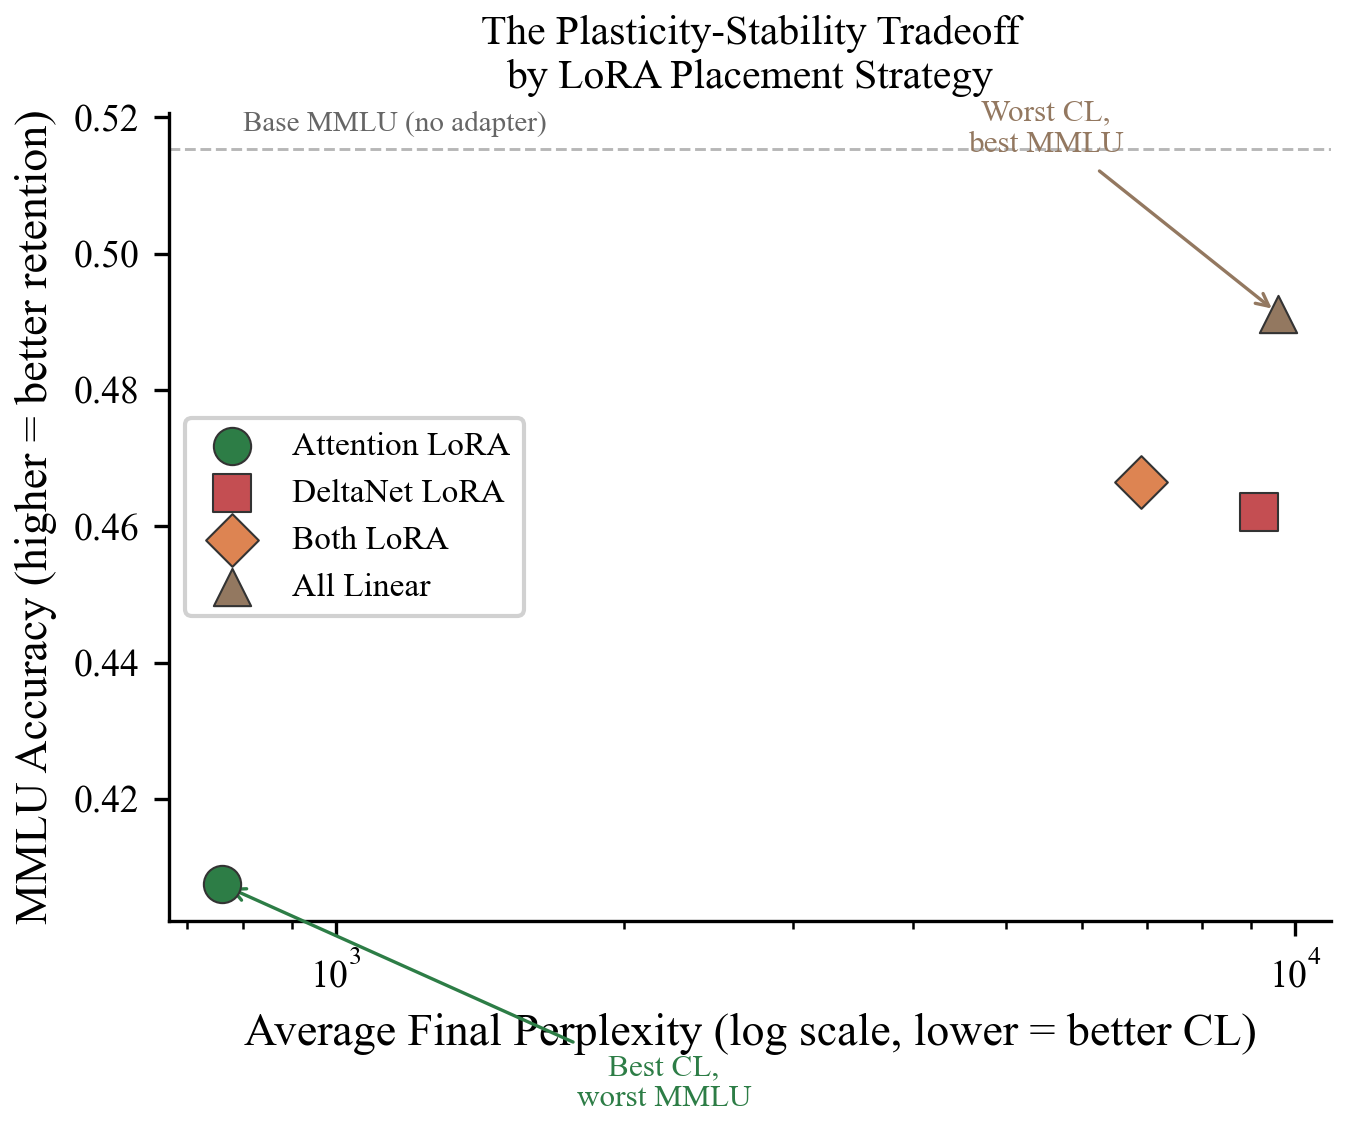
\includegraphics[width=0.8\textwidth]{figures/fig5_tradeoff_scatter.png}
\caption{The plasticity-stability tradeoff by LoRA placement. Attention LoRA (bottom-left) achieves the best CL performance but worst MMLU retention. All-linear (top-right) preserves general knowledge but fails at CL. No strategy achieves both.}
\label{fig:tradeoff}
\end{figure}

\subsection{Why Do Attention Layers Dominate CL?}

We hypothesize that the key-value attention mechanism provides a natural substrate for domain adaptation through LoRA. Attention layers compute:
\begin{equation}
\text{Attention}(Q, K, V) = \text{softmax}\left(\frac{QK^T}{\sqrt{d_k}}\right)V
\end{equation}

LoRA on $W_Q$ and $W_K$ adjusts \emph{what the model attends to}, while LoRA on $W_V$ and $W_O$ adjusts \emph{what information is extracted}. These are naturally composable across domains---attending to code syntax vs.\ mathematical notation requires different attention patterns but can coexist in the low-rank subspace.

In contrast, SSM layers (DeltaNet, Mamba) maintain a recurrent hidden state that integrates information sequentially. LoRA modifies the state transition dynamics, which is a more global perturbation---changing how the state evolves affects \emph{all} downstream tokens, making it harder to adapt to a new domain without disrupting previously learned dynamics.

\subsection{The Division of Labor in Hybrid Models}

Our MMLU results suggest a division of labor in hybrid models:
\begin{itemize}
    \item \textbf{Attention layers}: Adapting them provides high plasticity but degrades general knowledge, suggesting they are heavily involved in encoding factual and reasoning capabilities.
    \item \textbf{SSM layers}: Adapting them has little effect on CL or general knowledge, suggesting they primarily handle sequential dynamics and long-range context compression rather than factual storage.
\end{itemize}

This is consistent with the SSM-attention duality formalized by Dao and Gu \cite{dao2024mamba2}, where attention provides ``eidetic'' (exact) memory and SSMs provide ``fading'' (compressed) memory. We note that our results do not conclusively establish that attention layers \emph{store} general knowledge. An alternative explanation is that attention layers serve as a routing mechanism for knowledge stored elsewhere, and LoRA adaptation disrupts this routing, thereby degrading MMLU performance. Distinguishing between these hypotheses would require probing classifiers or representation analysis, which we leave for future work.

% ============================================================
\section{Limitations}

\begin{itemize}
    \item We evaluate on two hybrid architectures; results may differ for other designs (e.g., Zamba's shared-attention pattern, or models at 7B+ scale where CL dynamics may change \cite{biderman2024}).
    \item Our CL protocol uses a fixed domain order (Code$\to$Science$\to$Conversation$\to$Math). CL outcomes are known to be order-sensitive; testing multiple permutations would strengthen generalizability claims.
    \item MMLU evaluation uses 100 samples per subject on a single seed (seed 42), which may have wide confidence intervals. Full MMLU with multi-seed evaluation would provide stronger evidence for the plasticity-stability tradeoff.
    \item We use a single LoRA rank ($r=16$); rank sensitivity analysis (e.g., $r \in \{8, 16, 32\}$) is left for future work.
    \item The parameter counts differ across strategies (0.13\%--0.71\%), introducing a potential capacity confound. A parameter-matched comparison (e.g., attention LoRA at higher rank to match all-linear parameter count) would isolate the effect of layer type from adapter capacity.
    \item We do not compare against established CL mitigation strategies such as EWC \cite{kirkpatrick2017overcoming} or experience replay. Our focus is on layer selection rather than forgetting mitigation, but such comparisons would contextualize the absolute performance numbers.
\end{itemize}

% ============================================================
\section{Conclusion}

We present the first systematic study of LoRA placement in hybrid SSM-Attention models for continual learning. Our key finding is clear: \textbf{adapt the attention layers, not the SSM layers}. Attention-only LoRA achieves 9$\times$ lower perplexity than the next-best placement strategy and 12$\times$ lower than SSM-only adaptation, with 5.6$\times$ fewer trainable parameters than the standard all-linear approach.

However, this advantage comes with a tradeoff: attention adaptation erodes general knowledge ($-10.8$ percentage points on MMLU), while SSM adaptation preserves it but fails at CL. This reveals that attention and SSM layers play fundamentally different roles in hybrid models---attention layers are deeply entangled with general knowledge, while SSM layers are resistant to LoRA-based adaptation. These findings have implications beyond continual learning for any downstream adaptation of hybrid architectures.

\textbf{Practical recommendation:} For continual learning in hybrid models, use attention-only LoRA. If preserving general knowledge is critical, consider strategies that combine attention LoRA with knowledge preservation techniques such as regularization or knowledge distillation.

% ============================================================
\bibliographystyle{plainnat}

\begin{thebibliography}{25}

\bibitem[Hu et al.(2022)]{hu2022lora}
Edward~J. Hu, Yelong Shen, Phillip Wallis, Zeyuan Allen-Zhu, Yuanzhi Li, Shean Wang, Lu~Wang, and Weizhu Chen.
\newblock LoRA: Low-rank adaptation of large language models.
\newblock In \emph{ICLR}, 2022.

\bibitem[Jamba(2024)]{jamba2024}
AI21 Labs.
\newblock Jamba: A hybrid transformer-mamba language model.
\newblock \emph{arXiv preprint arXiv:2403.19887}, 2024.

\bibitem[Gu \& Dao(2023)]{gu2023mamba}
Albert Gu and Tri Dao.
\newblock Mamba: Linear-time sequence modeling with selective state spaces.
\newblock \emph{arXiv preprint arXiv:2312.00752}, 2023.

\bibitem[Yang et al.(2024)]{yang2024deltanet}
Songlin Yang, Bailin Wang, Yu~Zhang, Yikang Shen, and Yoon Kim.
\newblock Gated delta networks: Improving mamba2 with delta rule.
\newblock \emph{arXiv preprint arXiv:2412.06464}, 2024.

\bibitem[Qwen(2025)]{qwen2025}
Qwen Team.
\newblock Qwen3.5 technical report.
\newblock 2025.

\bibitem[Zamba(2024)]{zamba2024}
Zyphra.
\newblock Zamba: A compact 7B SSM hybrid model.
\newblock \emph{arXiv preprint arXiv:2405.16712}, 2024.

\bibitem[McCloskey \& Cohen(1989)]{mccloskey1989catastrophic}
Michael McCloskey and Neal~J Cohen.
\newblock Catastrophic interference in connectionist networks: The sequential learning problem.
\newblock In \emph{Psychology of Learning and Motivation}, volume~24, pages 109--165. Elsevier, 1989.

\bibitem[French(1999)]{french1999catastrophic}
Robert~M French.
\newblock Catastrophic forgetting in connectionist networks.
\newblock \emph{Trends in Cognitive Sciences}, 3(4):128--135, 1999.

\bibitem[Kirkpatrick et al.(2017)]{kirkpatrick2017overcoming}
James Kirkpatrick, Razvan Pascanu, Neil Rabinowitz, Joel Veness, Guillaume Desjardins, Andrei~A Rusu, Kieran Milan, John Quan, Tiago Ramalho, Agnieszka Grabska-Barwinska, et~al.
\newblock Overcoming catastrophic forgetting in neural networks.
\newblock \emph{PNAS}, 114(13):3521--3526, 2017.

\bibitem[Zenke et al.(2017)]{zenke2017continual}
Friedemann Zenke, Ben Poole, and Surya Ganguli.
\newblock Continual learning through synaptic intelligence.
\newblock In \emph{ICML}, pages 3987--3995, 2017.

\bibitem[Chaudhry et al.(2019)]{chaudhry2019tiny}
Arslan Chaudhry, Marc'Aurelio Ranzato, Marcus Rohrbach, and Mohamed Elhoseiny.
\newblock Efficient lifelong learning with A-GEM.
\newblock In \emph{ICLR}, 2019.

\bibitem[Serra et al.(2018)]{serra2018overcoming}
Joan Serra, Didac Suris, Marius Miron, and Alexandros Karatzoglou.
\newblock Overcoming catastrophic forgetting with hard attention to the task.
\newblock In \emph{ICML}, pages 4548--4557, 2018.

\bibitem[Dettmers et al.(2023)]{dettmers2023qlora}
Tim Dettmers, Artidoro Pagnoni, Aman Srivastava, and Luke Zettlemoyer.
\newblock QLoRA: Efficient finetuning of quantized language models.
\newblock In \emph{NeurIPS}, 2023.

\bibitem[Zhang et al.(2023)]{zhang2023adalora}
Qingru Zhang, Minshuo Chen, Alexander Bukharin, Nikos Karampatziakis, Pengcheng He, Yu~Cheng, Weizhu Chen, and Tuo Zhao.
\newblock AdaLoRA: Adaptive budget allocation for parameter-efficient fine-tuning.
\newblock In \emph{ICLR}, 2023.

\bibitem[Liu et al.(2024)]{liu2024dora}
Shih-Yang Liu, Chien-Yi Wang, Hongxu Yin, Pavlo Molchanov, Yu-Chiang~Frank Wang, Kwang-Ting Cheng, and Min-Hung Chen.
\newblock DoRA: Weight-decomposed low-rank adaptation.
\newblock In \emph{ICML}, 2024.

\bibitem[Wang et al.(2023)]{wang2023orthogonal}
Zifeng Wang, Zizhao Zhang, Chen-Yu Lee, Han Zhang, Ruoxi Sun, Xiaoqi Ren, Guolong Su, Vincent Perot, Jennifer Dy, and Tomas Pfister.
\newblock Learning to grow pretrained models for efficient transformer training.
\newblock In \emph{ICLR}, 2023.

\bibitem[Smith et al.(2023)]{smith2023continual}
James~Seale Smith, Leonid Karlinsky, Vyshnavi Gutta, Paola Cascante-Bonilla, Donghyun Kim, Assaf Arbelle, Rameswar Panda, Rogerio Feris, and Zsolt Kira.
\newblock CODA-Prompt: COntinual decomposed attention-based prompting for rehearsal-free continual learning.
\newblock In \emph{CVPR}, pages 11909--11919, 2023.

\bibitem[Dao \& Gu(2024)]{dao2024mamba2}
Tri Dao and Albert Gu.
\newblock Transformers are SSMs: Generalized models and efficient algorithms through structured state space duality.
\newblock In \emph{ICML}, 2024.

\bibitem[Yoshimura et al.(2024)]{mambapeft2024}
Masakazu Yoshimura, Teruaki Hayashi, and Yota Maeda.
\newblock Exploring parameter-efficient fine-tuning for Mamba.
\newblock In \emph{ICLR}, 2025. arXiv:2411.03855.

\bibitem[Nunez et al.(2024)]{hylora2024}
Elvis Nunez, Luca Zancato, Benjamin Bowman, Aditya Golatkar, Wei Xia, and Stefano Soatto.
\newblock Expansion span: Combining fading memory and retrieval in hybrid state space models.
\newblock \emph{arXiv preprint arXiv:2412.13328}, 2024.

\bibitem[Lu et al.(2024)]{codyra2024}
Haodong Lu et~al.
\newblock CoDyRA: Adaptive rank, reduced forgetting---knowledge retention in continual learning vision-language models with dynamic rank-selective LoRA.
\newblock \emph{arXiv preprint arXiv:2412.01004}, 2024.

\bibitem[Hayou et al.(2025)]{plop2025}
Soufiane Hayou et~al.
\newblock PLoP: Precise LoRA placement for efficient finetuning of large models.
\newblock \emph{arXiv preprint arXiv:2506.20629}, 2025.

\bibitem[Lopez-Paz \& Ranzato(2017)]{lopezpaz2017gem}
David Lopez-Paz and Marc'Aurelio Ranzato.
\newblock Gradient episodic memory for continual learning.
\newblock In \emph{NeurIPS}, pages 6467--6476, 2017.

\bibitem[Biderman et al.(2024)]{biderman2024}
Stella Biderman et~al.
\newblock Emergent and predictable memorization in large language models.
\newblock In \emph{NeurIPS}, 2024.

\end{thebibliography}

% ============================================================
\appendix
\section{Per-Domain Results}

\begin{table}[h]
\centering
\caption{Per-domain final perplexity after full CL sequence (Qwen3.5-0.8B, A100, seed=42).}
\label{tab:perdomain}
\begin{tabular}{lrrrr}
\toprule
\textbf{Strategy} & \textbf{Code} & \textbf{Science} & \textbf{Conversation} & \textbf{Math} \\
\midrule
Baseline (pre-CL) & 1.72 & 5.83 & 20.03 & 4.71 \\
Attention LoRA & 1,054 & 365 & 120 & 77 \\
Both LoRA & 17,340 & 2,326 & 1,041 & 4,448 \\
DeltaNet LoRA & 21,440 & 5,713 & 633 & 2,673 \\
All-linear & 17,907 & 5,112 & 5,997 & 17,220 \\
\bottomrule
\end{tabular}
\end{table}

\section{Training Details}

All experiments use AdamW optimizer with learning rate $2 \times 10^{-4}$, linear warmup over 10\% of steps, and batch size 4 with gradient accumulation of 4 (effective batch size 16). Maximum sequence length is 512 tokens.

Hardware: NVIDIA A100-SXM4-80GB (primary), NVIDIA L4 24GB, Apple M4 Pro (MLX). Total compute cost: approximately \$35 USD.

\end{document}
